\section{Genetic Operators}\label{sec:genetic_operators}
As has been mentioned, genetic operators are applied to members of an existing population to generate a new population. For this assignment the operators used included reproduction, crossover and mutation. As detailed by Koza and Poli \cite{koza2005genetic}, these operators can be briefly summarized as follows:

\begin{itemize}
    \item Reproduction: Copy the selected individual program to the new population as is.
    \item Crossover: Create offspring for the new population by combining randomly chosen parts from two selected programs.
    \item Mutation: Create one new offspring for the new population by randomly mutating a randomly chosen part of a selected individual.
\end{itemize}

Of course, these operators will not be used uniformly to generate new populations. Rather, every operator is associated with a probability which determines the likelihood that it will be used to select the next individual for the new population. Specifically, the probability for crossover was 0.9, the probability for mutation was 0.05 and the probability for mutation was also 0.05.

In addition, when applying operators decisions must be made regarding whether to select terminal (leaf) or non-terminal (internal) nodes. The probability for selecting a terminal node was chosen as 0.1 whereas the probability for selecting a terminal node was chosen as 0.9. 

Finally, a maximum tree depth of 16 was applied as a constraint to the individuals of a new population. In the case of crossover and mutation, the operators would not try to produce a valid individual more than once before failing.

With the selection methods and genetic operators having been identified, figure \ref{fig:breeding_pipeline} depicts the entire breeding pipeline for generating a new population from an existing population.

\begin{figure}[H]
\centering
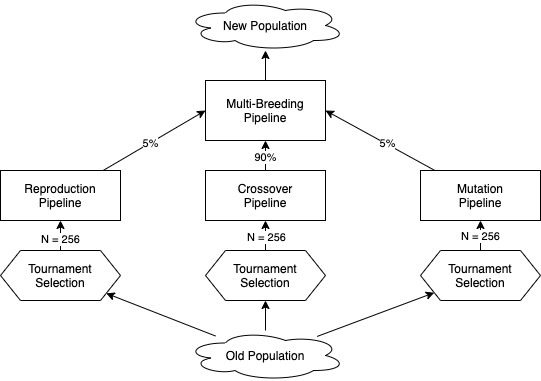
\includegraphics[width=\textwidth]{report/6_genetic_operators/breeding_pipeline.png}
\caption{Breeding Pipeling}
\label{fig:breeding_pipeline}
\end{figure}